\begin{center}
    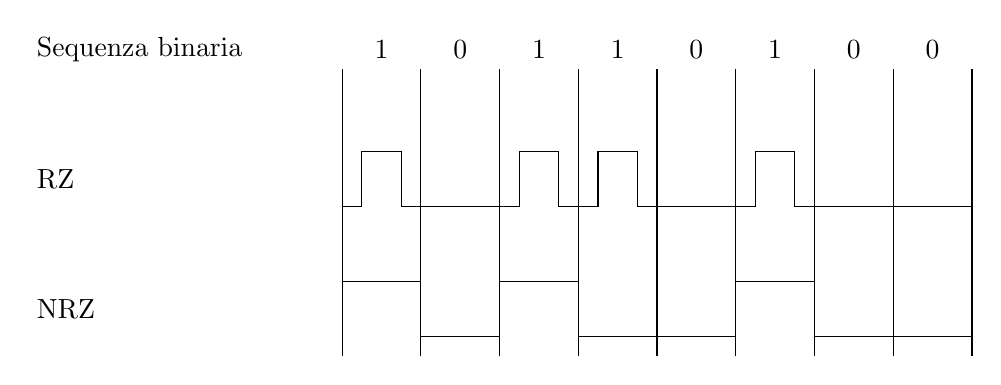
\begin{tikzpicture}
        %%%%%%%%% Barre %%%%%%%%%%
        \foreach \x in {4,...,12}
            \draw (\x,-0.25) -- (\x,3.4);
        
        %%%%%%%%% Numeri %%%%%%%%%
        \node at (4.5,3.65) {1};
        \node at (5.5,3.65) {0};
        \node at (6.5,3.65) {1};
        \node at (7.5,3.65) {1};
        \node at (8.5,3.65) {0};
        \node at (9.5,3.65) {1};
        \node at (10.5,3.65) {0};
        \node at (11.5,3.65) {0};

        %%%%%%%%%% NRZ %%%%%%%%%%%
        \draw (4,0.7) -- (5,0.7);
        \draw (5,0) -- (6,0);
        \draw (6,0.7) -- (7,0.7);
        \draw (7,0) -- (9,0);
        \draw (9,.7) -- (10,0.7);
        \draw (10,0) -- (12,0);

        %%%%%%%%%%% RZ %%%%%%%%%%%
        \draw (4,1.65) -- (4.25,1.65) -- (4.25,2.35) -- (4.75,2.35) -- (4.75,1.65) -- (6.25,1.65) -- (6.25,2.35) -- (6.75,2.35) -- (6.75,2.35) -- (6.75,1.65) -- (7.25,1.65) -- (7.25,2.35) -- (7.75,2.35) -- (7.75,1.65) -- (9.25,1.65) -- (9.25,2.35) -- (9.75,2.35) -- (9.75,1.65) -- (12,1.65);

        %%%%%%%% Legenda %%%%%%%%%
        \node[anchor=west] at (0,3.65) {Sequenza binaria};
        \node[anchor=west] at (0,2) {RZ};
        \node[anchor=west] at (0,0.35) {NRZ};
    \end{tikzpicture}
\end{center}